\chapter{Evaluation}\label{ch:eval}
Here I will evaluate:
\begin{enumerate}
  \item Findings from the FDC investigations
  \item Compare the proposed active vision approaches to non-active systems from before
\end{enumerate}\todo{split later if needed}

% Setuo
\section{Evaluation Setup}
The general setup included training a set of policies with their inherent hyperparameters, which will be discussed during their specific sections.

\subsection{Collected Data}
The data I chose to collect to reason about these policies are:
\begin{itemize}
  \item \textbf{Camera Type} A misnomer, indicates which sensors or combinations of sensors are being used in the policy to make decisions from \({RGB}_{wrist, ~left\_shoulder, ~right\_shoulder}\) and \(Depth_{wrist}\).
  \item \textbf{Final Distance} (to target) all of my tasks are target centric, so final distance within the allowed episode length a measure of competence.
  \item \textbf{Minimum Distance} (to target) as above. The difference is reasoning where a policy might be falling apart, seeing the discrepancies between \emph{min} and \emph{final}
  \item \textbf{Success Rate} All the tasks had slightly differing success criteria, however this is an important measure for competency again. This was mostly measured as a count out of $n$, for $n$ being the length of the test demonstrations. The term ``test demonstrations'' means that a set of demos were recorded with the target and the environment in a fixed state. Loading these back allows us to hae a comparable test between policies and their variables.
  \item Other policy specific hyperparameters that were relevant to observe. These will be discussed when relevant.
\end{itemize}

\subsection{Reproducibility and Verification}
All the random aspects that can be controlled, be it \emph{numpy} and \emph{pytorch} random choices or random `live' demos. Seeds are sets for both the libraries, as well as the \verb|DataLoader| seeds being fixed for the entirety of the policies tested here.
The demos per task are pre-made and saved in the project repository. \todo{ref the final deliverables bit}. I repeated all the tests with $5$ different seeds for the data shuffling, to observe if training on a different (but controlled) ordering of the demos affects a policy.

\section{Test Environments}
Two main branches of tasks I followed in this project are grasping and occluded reaching tasks.

\subsection{Reaching with an Obstacle - \textbf{ReachObs\_Random}}

\textbf{ReachObs\_IndRandom} is not discussed here in depth, due to the similarity of the tasks, and the independent version not being any more interesting. Some results for this test can be found here\todo{add appendix}.

\subsection{Grasping}
These two grasping tasks are to assess the contextual 3D understanding of the policy: learning depth information and adapting to differing sizes of targets; as well as learning the workspace before attempting a task \todo{grasp then move, not sure if I have time for this, but If i do defo interesting}

\subsection{Grasp and Depth Understanding - \textbf{Vision\_Random}}
This task is quite similar to the depth interfacing tests from earlier.\todo{ref DI}. The main difference is that the placement of the targets are random within he workspace, for \emph{training}, \emph{control} and \emph{test} sets. The test is repeated with different sizes of targets, \textbf{normal} and \textbf{smaller} (target scale is half that of normal). The training and the control sets are the same size while the test will be the the other. The reasons for this is to assess:
\begin{enumerate}
  \item The effectiveness of the configuration in solving the task it is immediately trained for
  \item Assess the information extraction from the various views by comparing the discrepancy between control and test.
\end{enumerate}
I created two separate variations of this specific task. One where the training and control set is set to be the \textbf{normal} size and we evaluate that on \textbf{smaller} blocks. The next variation is flipping this configuration: control and training are scaled down, while test is normal sized. Mainly to investigate whether the information wew train on has any affect on the policy proficiency.

\textbf{Important Note!}
The demos saved for all the configurations are tested and checked to appear correctly. However, I have realised that the specifically the \textbf{saved smaller testing demos} which is used in the place of the control or the test, would spawn three of the targets smaller than they need to be. Index 2, 5, 6 \todo{confirm this!} will spawn smaller and hence look smaller. It might be valid to remove these from the later numbers as they might affect the overall success rates of smaller tasks. 

I have not figured out the reasoning for this, it has happened before and no effort to fix this issue as resolved, I speculate that it is an issue with how I control the sizes of targets. The target size is set during the start of an episode, so this means the \verb|Environment| object from PyRep must be either initialising an episode wrong from the way it is saved. This was not an isolated accident with the saved demos, it would happen every once in a while, which means that the issue must have happened during saving the smaller demos. Because the problem is consistently repeated. This should not affect the training, as this set was confirmed to spawn correctly. The evaluation of the results will have to take care of this fact.


\subsection{Carrying the Target - \textbf{Grasp\_ThenMove}}\todo{havent run this yet, might remove it depending on what I will do today}

\section{Evaluated Configurations}\todo{not sure about this maybe talk about these per task down the line}

% Naive Cam-Attention (from reach-obs)
\section{Naive Colour Attention - Results}
This is the results relating to the proposed naively active approaches from \ref{sec:reach-obs-naive-cam-attn}.
The variations of this policy I tested included: \todo{add code for aall the possibilies from test cam attn py file}
\begin{itemize}
  \item Separate or joint Feature Encoders (\verb|is_multi_cnn|)
  \item \emph{mean} or \emph{max} pooling for the colour score (\verb||)
  \item $\lambda_{attn}$ loss parameter that scales the KL divergence of the predicted 
  weights.
\end{itemize}
These were tested over multiple RGB camera combinations, namely:
\begin{enumerate}
  \item Wrist, Left Shoulder and Right Shoulder
  \item Wrist and Right Shoulder
  \item Wrist and Left Shoulder
  \item Left and Right Shoulder
\end{enumerate}
No single camera was tested, as the idea of this policy is to investigate the interaction between cameras and their features.

Finally, they were tested for increasing epochs in \(\left[100, ~200, ~500, ~1000, ~2000\right]\) to observe longer training trends.

The policies were trained on the first 10 of the saved demos under \todo{put the repo data link, and add to appendix} and tested on the 10 test demos saved under \todo{again same, copy link etc}.

Finally, I collected the attention weights for the different cameras during the episodes and 

\subsection{Observations}
The main takeaway from this task was how it favoured longer epochs of training. The most success and lowest distances to target were recoded in the $500$ to $1000$ range, then the success rate starts decreasing again, meaning overtraining and no more benefit.\todo[color=purple]{}

The very likely reason for this is that, the demonstration trajectories for this task are a lot more varied due to the obstacle. More importantly the choice to move around the obstacle, there are demos that force the arm to go to the left go back and down, or left then down. This high variation means the agent needs longer time to average out motions in strict Behavioural Cloning settings, and takes longer.
\todo{show the attn lambda  = 5 results}


\subsubsection{Separate Feature Encoders}
This parameter was more of a test to see if it interacted well in any way. Theoretically both approaches are sound. 

This task is quite unforgiving and errors add up quickly, if the robot gets stuck on the obstacle, it rarely manages to save itself. Evident from the quick increases in minimum distance between epochs $100$ and $200$ for single-CNNs, which capture early fitting due to information abundance, but get confused trying to generalise due to the feature encodings keeping a lot of this uncertainty.

Conversely, multi-CNNs learn late. Makes sense as more passes allow each CNN (now seeing only one frame not all) to learn slowly. Therefore, the multi-CNN policies have a more decisive dip in minimum distance reinforcing the idea that training for loner allows them to capture pose specific information that is helpful to the system in solving this task.

The only interesting remark here is that multi-CNN interacts interestingly with \emph{mean} pooling. Seeing the spiky and jagged Single-CNN graphs we can confirm speculate that merging all views and convoluting them likely confuses the feature extraction and a lot of uncertainty creeps in to the features.


\subsubsection{\emph{Mean} and \emph{Max} Pooling}
\todo{obseration, put some min dist here}
The differences here are extremely subtle. General observations both work fairly similarly in terms of the minimum distance they can reach per epoch. A stark difference, however, is how jagged and uncertain \emph{max} is with lower epochs. This is due to max likely sending a similar signal between all views, if more than one view can see the target, they will likely have very similar weights. Which can add indecisiveness, especially when both shoulders are active.

\emph{Mean} is not necessarily any better when single-CNNs are used. Again, due to uncertainty creeping in, but from the view understanding.

Though, its performance immediately starts good when it is paired with multi-CNN feature encoder. This makes the data less spread out \todo{looking at the minimum dist graphs here} and the policy being capable of moving past the target, even from the start. However, the drawback is, the performance does not get much better for shoulder cameras as training goes on. This is now likely due to how \emph{mean} operates, it relates the score magnitude to depth essentially, more area covered the better. The shoulder cams being at a fixed depth, don't allow them to participate in this benefit. So \emph{max} with Multi-CNN combination is generally more successful than \emph{mean} with combinations using shoulder cams.

\subsubsection{Attention Loss Weights ($\lambda_{attn}$)}
This didn't seem to make a change at all. However, looking at the loss curves \todo{add a loss curve here, fighting for vram currently}, some potential issues may be that the one loss term is drowning the other one out and scaling it up might not matter, rerun depending on this.


\subsubsection{Remarks}
I thought this policy would be able to fix the shortcomings, which was the final reach toward the obstacle not being executed well. Non-wrist cameras help with the first half of the motion while the wrist camera should be able to generalise to the final reaching motion \todo{explain: due to its self-centric nature}. However the problem is the demos don't force the gripper to `look' towards the target. So, the wrist camera cannot get the benefits from a \emph{mean} pooled configuration. This led to the attention weights being very similar above and below the obstacle. Which counteracts this policy's theoretical benefits.



\section{Multi-Modal Results}

  \subsection{Baseline - Naive Modality Concatenation}
This will be the baseline to compare the rest of the data. A hard set hyperparameter is the encoding CNN, for which the code can be found here \todo[color=green]{appendix code}. The layers of which are set to $\left[32, ~48, ~64, ~128\right]$ and the final encoding is of shape \(\langle 128, ~2, ~2 \rangle\).


\subsubsection{Grasp}
\begin{figure}[htpb]
  \centering
  
\includegraphics[width=\linewidth]{assets/evaluation/baseline/base-grasp-final.png}
  \caption{Final Distances Reached for the Grasp task}\label{fig:base-grasp-final}
\end{figure}

\begin{figure}[htpb]
  \centering
  \includegraphics[width=0.6\linewidth]{assets/evaluation/baseline/base-grasp-control-success-cams-epochs.png}
  \caption{Success Rate (\%) of task per cam type over epochs}\label{fig:base-grasp-control-success}
\end{figure}
The `test' counterpart had no successes.


\subsubsection{Reach with Obstacle}



  \subsection{Separated Understanding of Depth}
This section is comparing the simple, yet more nuanced fusing techniques introduced in \todo{ref to policies}. Parameters set can be found in Table \ref{tab:sep-dep-params}.

\begin{table}[H]
\centering
  \begin{tabular}{|| c | c | c ||}
  \hline
  Flavour & Parameter & Value \\
  \hline
  
  \multirow{2}{*}{CNN Encoder Module} & rgb\_layers & [32, 48, 64, 128] \\
  & depth\_layers & [32, 48, 64, 128] \\
  \hline
  \multirow{3}{*}{Cross Attention Module} & embed\_size & 128 \\
  & num\_heads & 8 \\
  & deep\_fuse & \texttt{True} \\
  \hline
  \end{tabular}\caption{Default Training parameters}\label{tab:sep-dep-params}
\end{table}

\subsubsection{Grasp - Normal}
The distributions of final distance is almost identical to the baseline, as they use similar methods and similar convolutions to extract features. The final distance comparison can be found here \todo{appendix}. However, an interesting observation was in the success rates of the tasks Figure \ref{fig:sepdep-normal-success}, where the control success rate more than quadruples the baseline (indicated in blue) at best and at least 37\% better than it in the `control' setting. For both separately fusing the the depth running cross attention on the depth and the rgb features when only the wrist modalities are included.

These being more successful, and greater in magnitude to success rates when any shoulder camera is included means that the task is solvable completely by just wrist modalities and the shoulder cameras are just confusing the grasp decision by diluting the data pool.\todo[color=purple]{diluting the data pool}

So the two best 

\begin{figure}[H]
  \centering
  
\includegraphics[width=\linewidth]{assets/evaluation/sep-dep/grasp-normal-success-cams.png}
  \caption{(Grasp Success Rate\textbf{normal})}\label{fig:sepdep-normal-success}
\end{figure}

\subsubsection{Grasp - Smaller}
The smaller results were identical to the baseline results. The reason is likely the difficulty of learning the smaller grasp task, and the network being tuned to learn the larger task inhibits its ability to perform here. Results are provided in \todo[color=green]{appendix}. Therefore, for higher success rates in the `test' configuration we should tune for it separately. Which highlights the difficulty in creating a single policy to cater to all tasks. Even smaller deviations are causing huge hurdles in learning.

\subsubsection{Reach Obs}
Somewhat similarly to the grasp tasks. The distances reached are identical within a small error. \todo{appendix} However, a big difference is the success rate (Figure \ref{fig:sep-dep-reach-success}) of the system, which surprisingly is either just about on par or worse than the baseline (included in blue). This means that the separate learning of depth information and later fusion helps the separate grasp\verb|grasp_head| to learn to grasp better than the baseline, yet they add no benefit in the reaching case.

\begin{figure}[H]
  \centering
  
\includegraphics[width=\linewidth]{assets/evaluation/sep-dep/reach-success-cams-epochs.png}
  \caption{Reach success rates per cam type}\label{fig:sep-dep-reach-success}
\end{figure}

  
  \subsection{Wrist Modulation - FiLM}\todo{wwaaffle more coherently, relate to depsep}
The results here are following the proposed modulation 6 wrist RGB and depth modulation techniques from Section \ref{subsec:policies-film}. Each variant of this policy has some hyperparameters associated with it. I landed on using the following after preliminary testing reasoning and about the structure of the data.The baseline is included in plots(in blue) is also included in the plot for easy comparison. 

\noindent For \textbf{LATE} models, with the initial learnt down-sampling and the FiLM module
\begin{itemize}
  \itemsep0em
  \item Initial Downsampling Network, which does $3$ convolutions takes in a \(\langle 3, ~64, ~64 \rangle\) image and returns features of shape \(\langle 16, ~4, ~4 \rangle \)
  \item Then the FiLM module takes in two of these feature vectors and does the modulation. The resulting encoding size is \(16 \times 4 \times 4 = 256\) as FiLM does change the shape of the given tensor.
  \item If there is bi-modulation the final encoding is double the size, $512$, as the modulated vectors are concatenated.
\end{itemize}

\noindent For \textbf{NON-LATE} models:
\begin{itemize}
  \itemsep0em
  \item Shallow encoder, used to match the channel dimension of modalities, is a single \verb|Conv2d|  that upsamples the channel dimensions to $6$ while preserving width and height ($64 \times 64$), \todo[color=green]{again appendix}.
  \item The FiLM network as before does not change the sizes returns \(\langle 12, ~64, ~64 \rangle \) or \(\langle 6, ~64, ~64 \rangle \) respectively if it is bi-modulation or not.
  \item Finally there is another CNN that encodes these modulated features, see \todo[color=green]{appendix}, which have layers $\left[36, ~72, ~128, ~128\right]$ and $\left[32, ~48, ~64, ~128\right]$ respectively to bi or not. The final feature size is \(\langle 128, ~2, ~2 \rangle\) regardless.
\end{itemize}


\subsubsection{Grasp}
Immediate observations from, Figure \ref{fig:film-grasp-final}, is that any modulation, reaches the similar final distances both the wrist and the wrist and depth data was reaching beforehand in the baseline. \textbf{Early} modulation seems to be more effective in understanding the `control' task so learning the trained distribution, where depth modulated RGB (\verb|Wdilm_D|) gets as close as the baseline. Although the other way around, seems be the worst of the bunch. THis must be due to the information richness in the RGB view, so the chunked linear layer within the FiLM network might not be able to accurately capture the required $\gamma$ and $\beta$ leading to the subpar performance seen here ($\approx 0.29$), around double the minimum distance the baseline can reach ($\approx 0.17$). While \textbf{late} modulation not only more successful at grasping the target Figure \ref{fig:film-grasp-success}, but also reaches closer to the `test' sample. 

Success of early modulation is also higher than the baseline \ref{subfig:base-grasp-control-success-smaller}. However, the `test' grasping is no better. Even though the late modulated version have some chance and that is better than the baseline, the puny 1-2\% could be attributed to random chance \todo[color=red]{compare the grasp attempts of these, if there are more grasp attempts but failures it is not random chance but better learning of wwhen to grasp, but the mvement is bad (late does not reach asclose, so maybe grasping is good, but do a table of grasp attempts versus successful grasps??)}

\begin{figure}[H]
  \centering
  
\includegraphics[width=\linewidth]{assets/evaluation/film/film-grasp-final.png}
  \caption{Final Distances Reached for the Grasp task \textbf{normal}}\label{fig:film-grasp-final}
\end{figure}\todo[color=red]{include the baseline wrist rbg+depth line in this graph}

\begin{figure}[H]
  \centering
  \begin{subfigure}{0.45\linewidth}
    \centering
    \includegraphics[width=\linewidth]{assets/evaluation/film/film-grasp-success.png}
    \caption{Grasp success per epoch and over seeds for `Control' and `Test'}\label{subfig:film-grasp-success}
  \end{subfigure}
  \hfill
  \begin{subfigure}{0.45\linewidth}
    \centering
    \includegraphics[width=\linewidth]{assets/evaluation/film/film-grasp-control-success-epochs.png}
    \caption{Success for `Control' per Epoch (shared legend)}\label{subfig:film-grasp-control-success-epoochs}
  \end{subfigure}
  
  \caption{Grasp Success for the FiLMed configurations}\label{fig:film-grasp-success2}
\end{figure}\todo{tabify this list}


\begin{table}[ht]
\centering
  \begin{tabular}{||c c c||}
  \hline
  Check Type & Avg Attempts for Success & Avg Attempts for Failure\\
  \hline
  \hline
  \multicolumn{3}{||c||}{\textbf{normal}} \\
  control & 1.23 & 1.21 \\
  test    & 1.00 & 2.75 \\
  \hline
  \multicolumn{3}{||c||}{\textbf{smaller}} \\
  control & 4.40 & 0.94 \\
  test    & 1.03 & 1.08 \\
  \hline
  \end{tabular}\caption{Grasp Attempts and Success}\label{tab:film-grasp-attempts}
\end{table}

We finally have a module that seems to improve its success rate, Figure \ref{fig:film-grasp-success}. While the distance distribution still seems to be similar to the baseline \ref{fig:film-grasp-final-smaller}. This is probably because when the task is not successful the arm will move around a bit more and potentially move slightly away. The 10cm is still within the grippers view range, the wrist camera i mounted around 8cm form the gripper tip. Although the `test' (now \textbf{normal}) is more better the `control' is not benefiting from this \ref{subfig:film-grasp-control-success-epoochs}. I think this is only  due to the smaller target being tougher to grab. if the gripper does not fully align with the target the grasp is almost always unsuccessful. \todo{include some grasping pictures here??}


\begin{figure}[H]
  \centering
  
\includegraphics[width=\linewidth]{assets/evaluation/film/film-grasp-final-smaller.png}
  \caption{Final Distances Reached for the Grasp task \textbf{smaller}}\label{fig:film-grasp-final-smaller}
\end{figure}

\begin{figure}[H]
  \centering
  \begin{subfigure}{0.30\linewidth}
    \centering
    \includegraphics[width=\linewidth]{assets/evaluation/film/film-grasp-success-smaller.png}
    \caption{Grasp success per epoch for `Control' and `Test'}\label{subfig:film-smaller-grasp-success}
  \end{subfigure}
  \hfill
  \begin{subfigure}{0.30\linewidth}
    \centering
    \includegraphics[width=\linewidth]{assets/evaluation/film/film-grasp-control-success-epochs-smaller.png}
    \caption{Success for `Control' per Epoch (shared legend)}\label{subfig:film-grasp-control-success-epochs}
  \end{subfigure}
  \hfill
  \begin{subfigure}{0.30\linewidth}
    \centering
    \includegraphics[width=\linewidth]{assets/evaluation/film/film-grasp-test-success-epochs-smaller.png}
    \caption{Success for `Test' per Epoch (shared legend)}\label{subfig:film-grasp-test-success-epoochs}
  \end{subfigure}
  
  \caption{Grasp Success for the FiLMed configurations}\label{fig:film-grasp-success}
\end{figure}


\subsubsection{Reach with Obstacle}
The heightened depth understanding capabilities are also seen here \ref{fig:film-reach}. The minimum distances reached by the FiLM policies are all below the obstacle and closer than the baseline. In the grasping task, double modulation seems to perform better. However, in the reaching task ``Colour modulated Depth'' variants (\verb|W_Dfilm{_LATE}|) are clearly more successful. I suspect this is because of the obstacle, understanding where it is in relation to the wrist only benefits the learning.

\begin{figure}[htpb]
  \centering
  \begin{subfigure}{0.40\linewidth}
    \centering
    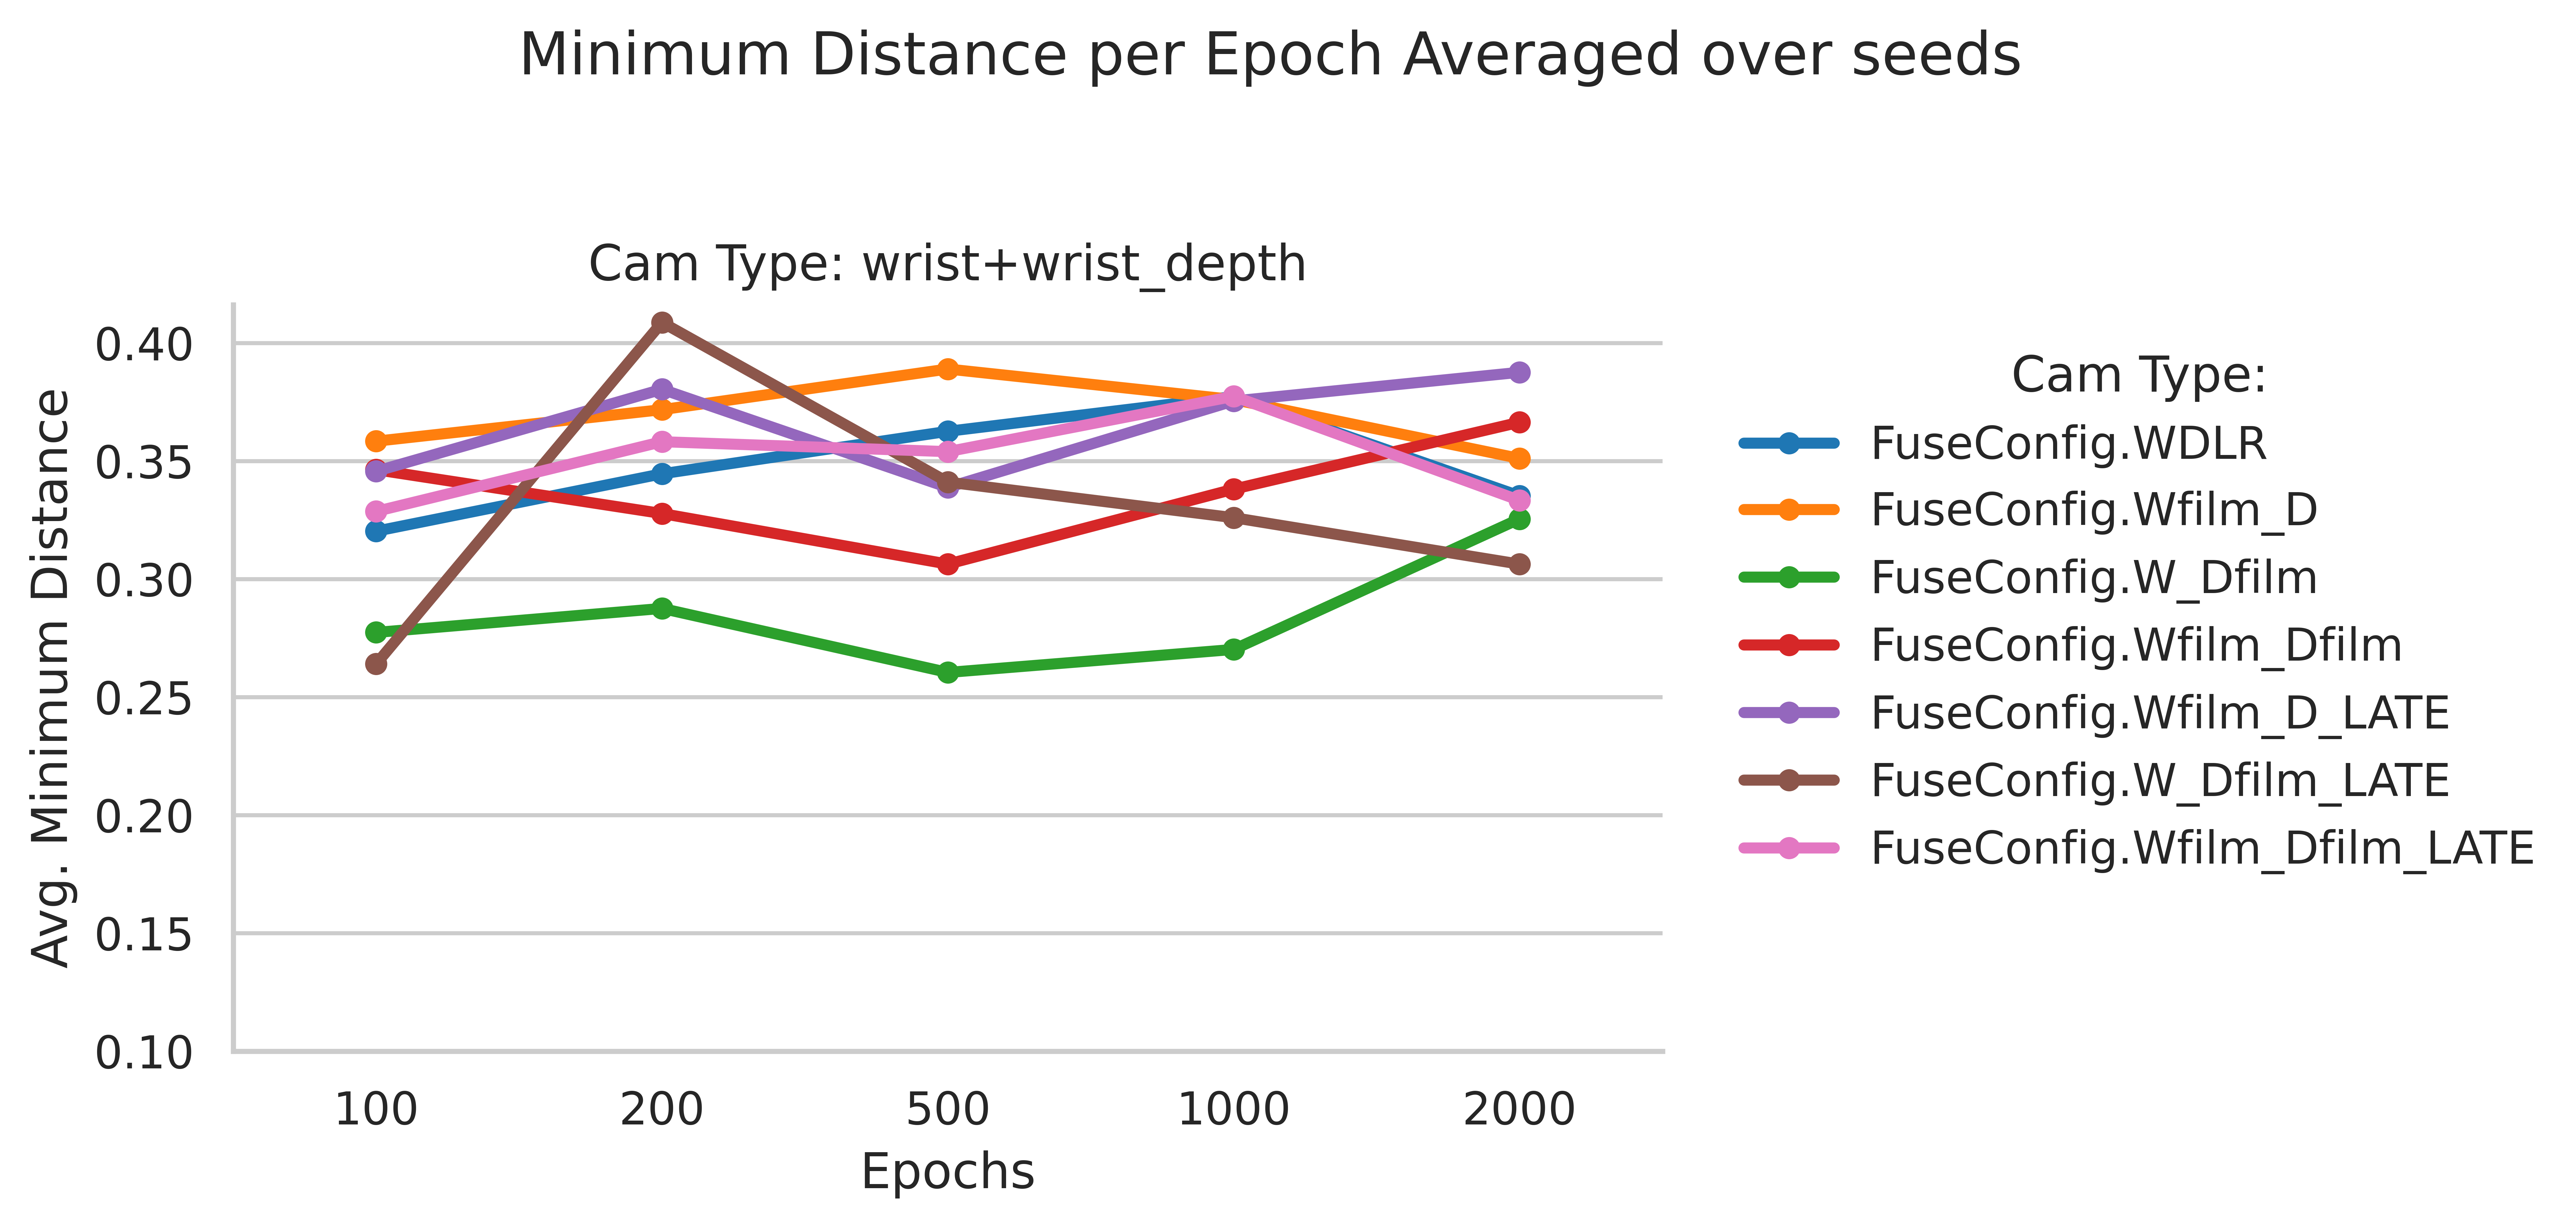
\includegraphics[width=\linewidth]{assets/evaluation/film/reach-min-cams.png}
    \caption{Minimum Distance tor reach target}\label{subfig:film-reach-min}
  \end{subfigure}
  \begin{subfigure}{0.40\linewidth}
    \centering
    \includegraphics[width=\linewidth]{assets/evaluation/film/base-reach-success-config-epochs.png}
    \caption{Reach Success Rates per Epoch}\label{subfig:film-reach-success}
  \end{subfigure}
  \caption{Reach Results}\label{fig:film-reach}
\end{figure}



  \subsection{Derivate Methods}
There are again some tuned parameters in this section, see Table \ref{tab:derivative-params}.

\begin{table}[H]
\centering
  \begin{tabular}{|| c | c | c ||}
  \hline
  Flavour & Parameter & Value \\
  \hline
  \multirow{1}{*}{MultiCNN} & rgb\_layers & [32, 48, 64, 128] \\
  \hline
  \multirow{1}{*}{4-way FiLM} & downscaling\_cnn & [32, 48, 64, 128] \\
  \hline
  \multirow{3}{*}{4-way Multi View Attention} & embed\_size & 128 \\
  & num\_heads & 8 \\
  & num\_layers & 4 \\
  \hline
  \end{tabular}\caption{Default Training parameters}\label{tab:derivative-params}
\end{table}

\subsubsection{Grasp Normal}
This section
\begin{figure}[H]
  \centering
  
\includegraphics[width=\linewidth]{assets/evaluation/derivatives/grasp-normal-wd.png}
  \caption{Wrist and depth}\label{fig:deriv-normal-final-wd}
\end{figure}

\begin{figure}[H]
  \centering
  
\includegraphics[width=\linewidth]{assets/evaluation/derivatives/grasp-normal-allcams.png}
  \caption{}\label{fig:deriv-normal-final-allcams}
\end{figure}

\begin{figure}[H]
  \centering
  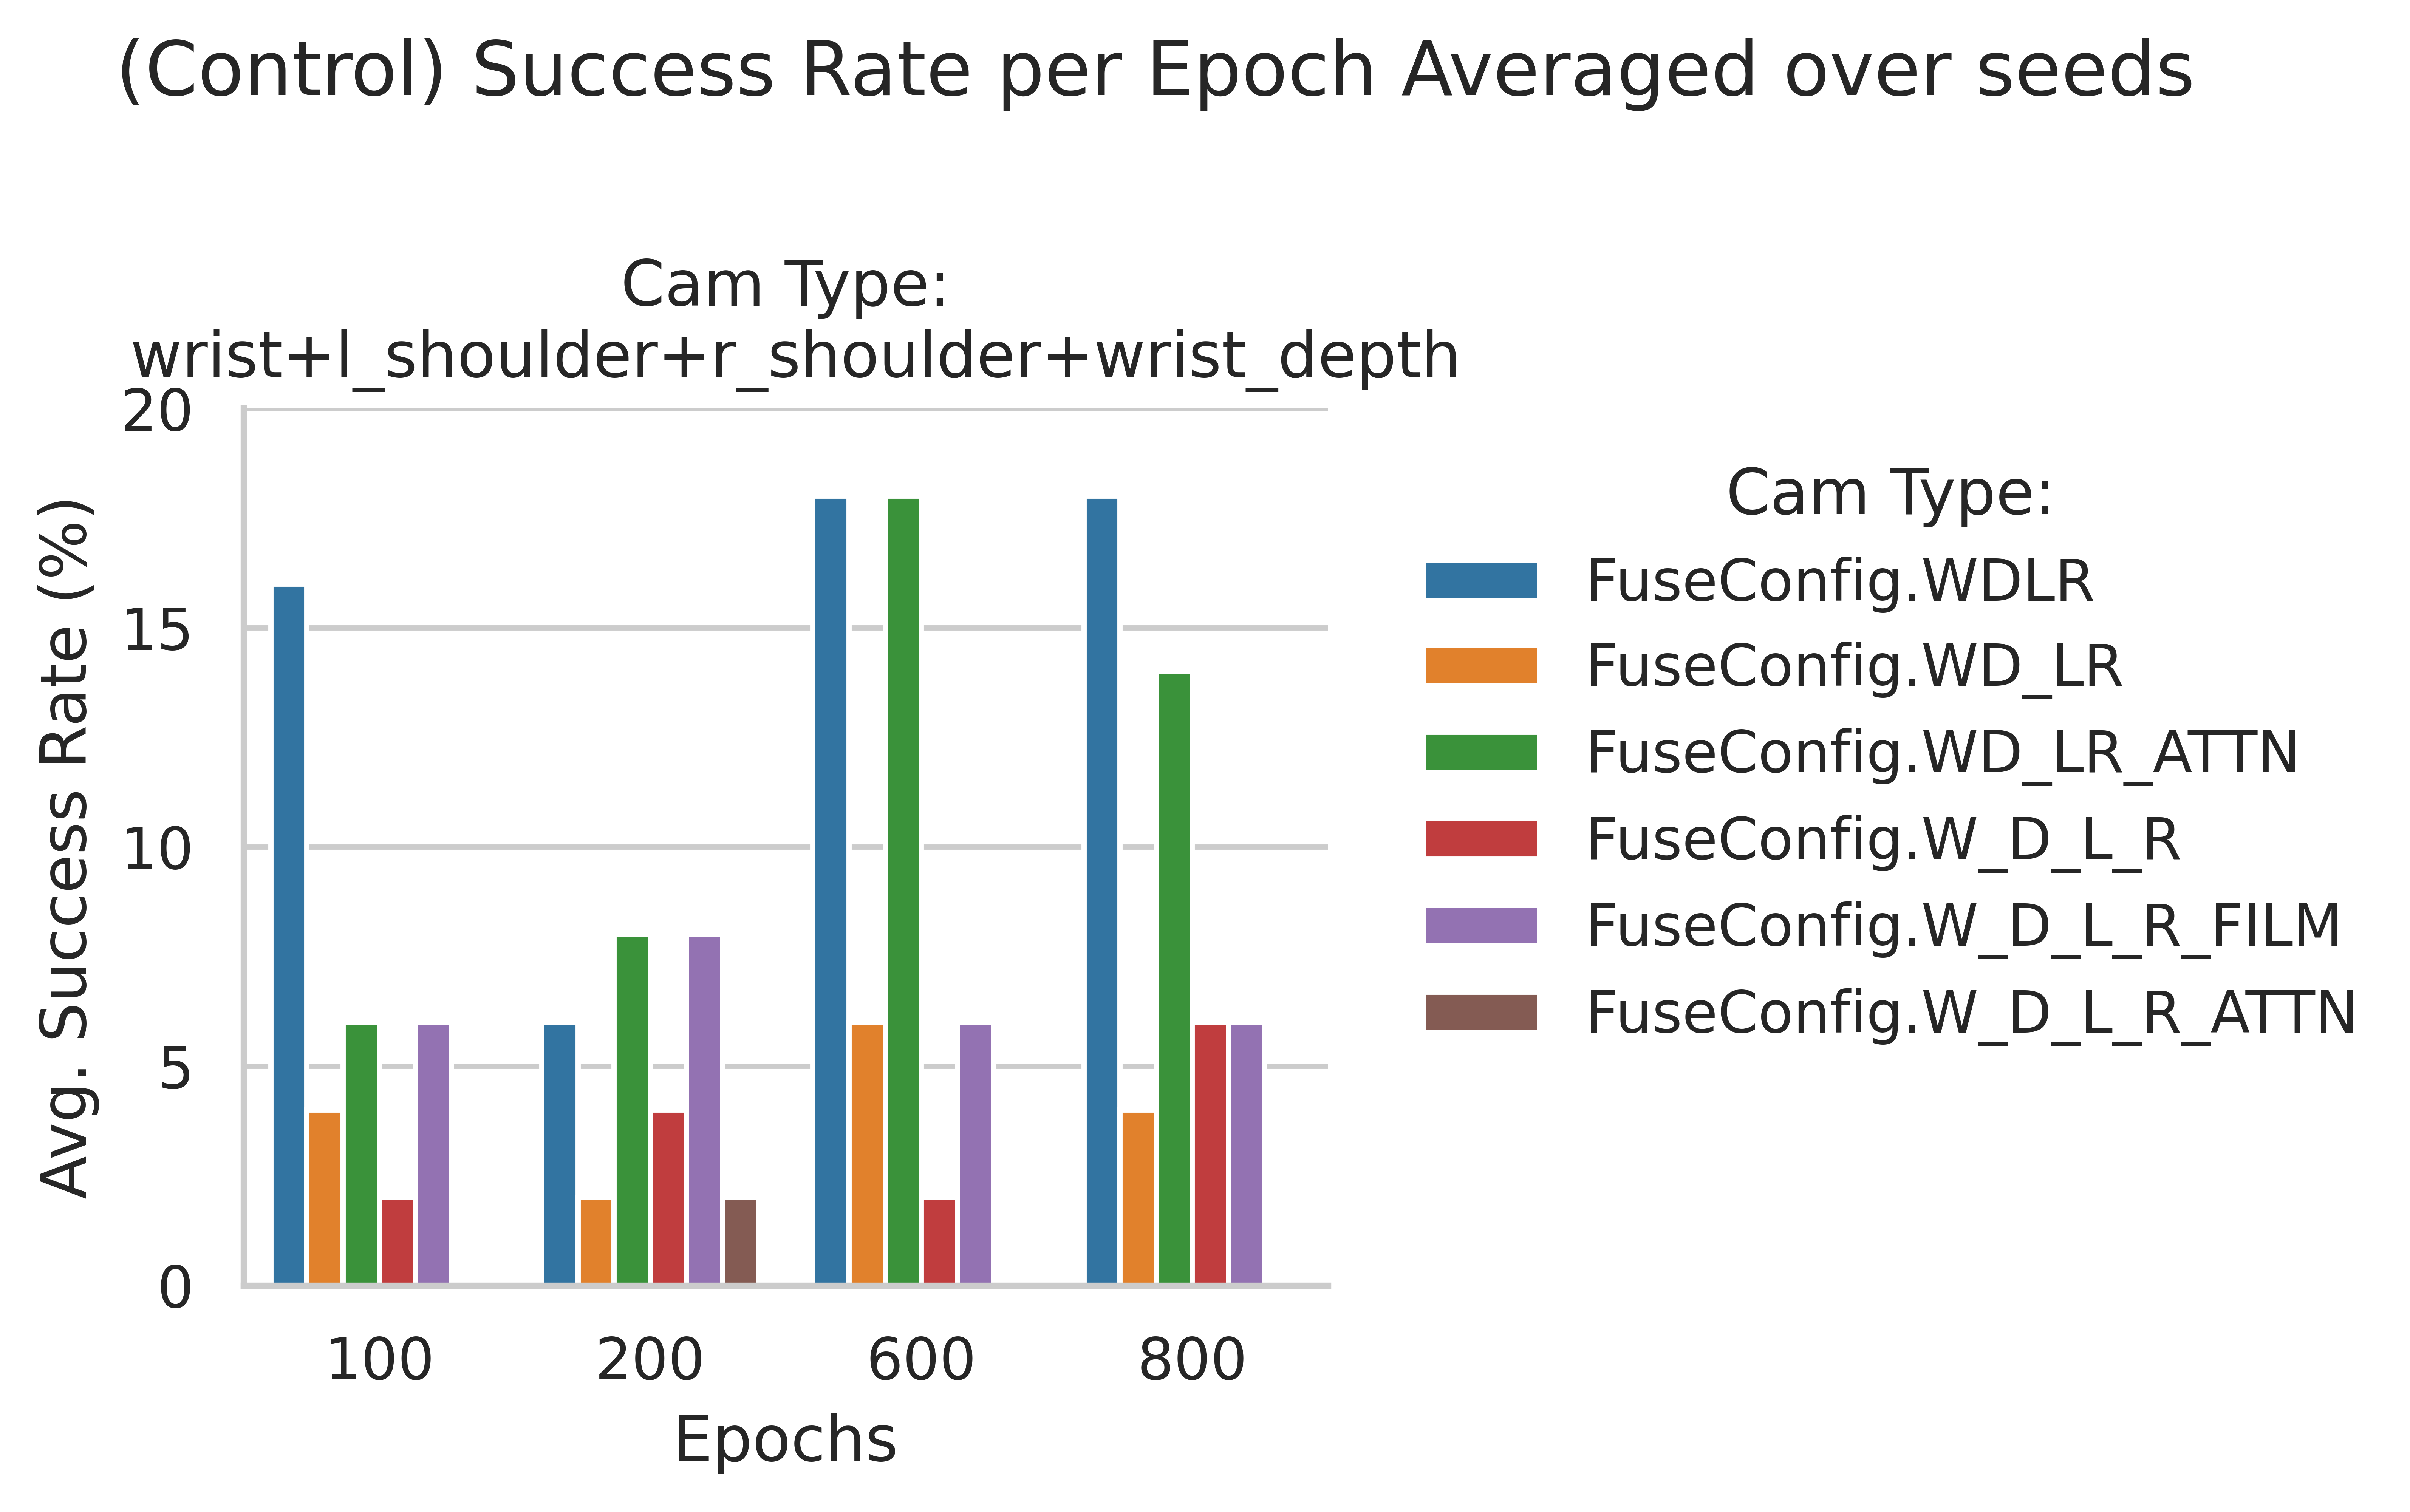
\includegraphics[width=\linewidth]{assets/evaluation/derivatives/grasp-normal-control-success-cams.png}
  \caption{}\label{fig:}
\end{figure}

There is not success for the `test' run!

\subsection{Reach}

  \subsection{Recurrent Models}
Quite differently I started with tuning a possible RNN model. There were too many variables to be running different epoch configurations and getting a fine-tuned definite answer would be difficult. Some parameters that are frozen can be found in Table \ref{tab:rnn-params}.

\begin{table}[ht]
\centering
  \begin{tabular}{|| c | c ||}
  \hline
  Parameter & Value \\
  \hline
  \multirow{2}{*}{input\_size} & 512 \\
  & \emph{or the fusion encoding size} \\
  \hline
  hidden\_size & 256\\
  num\_layes & 1 \\
  batch\_first & \texttt{True} \\
  bidirectional & \texttt{False} \\
  \hline
  \end{tabular}\caption{LSTM initialisation parameters}\label{tab:rnn-params}
\end{table}

\subsubsection{Baseline Tuning}
I started with experimenting with the baseline. Planning to find the most promising training length before I applied the promising fusion methods to architecture. Looking at the final distance distributions for various epochs in Figure \ref{fig:rnn-grasp-final-wd}, I realised that the most promising models were trained were generally shorter durations and $400$ to the $600$ epochs mark. These were optimal in reaching, getting around the 11 cm mark from the object. However, their grasp success was troubling, wrist RGB and the depth together were successful around 8\% - 10\% while the others were not grasping at all.

Then including the different views, Figure \ref{fig:rnn-grasp-tuning}, it is clear that the wrist combinations act better with shorter training, though, wrist and wrist depth together hangs behind quite a bit. This is likely due to consistent motion patterns the task as well as the easy distributional alignment the wrist cameras inherently produces. It is surprising that the inclusion of the depth camera struggles, bringing the density around 2.1 and having a more prominent second peak at 0.45 metres. These are likely due to the `test' data, however, gives another insight into to the non-optimal nature of the data fusion of the baseline.

Shoulder combinations however, heavily favour longer training, though not too long. Likely due to the smaller Signal-to-Noise (SNR) ratio. There is just more extraneous data captured by the shoulders and that takes the model longer to fit to it. However, once fit 600 epochs of training, it seems to reach the 0.14 mark more often. 

A final qualitative observation I had was the movement competency. Although hard to convey here, observing the robot its movement less spiky, and more than once I observed a smooth trajectory change. It would first start off, doing a generic reach, then around half way around the movement slow down, slightly reposition and reach for the target very competently. I speculate this is the hidden LSTM states coming in handy and providing that encapsulated information of the state the robot is in currently. Allowing it to do BC with episode length awareness like never before.

\begin{figure}[H]
  \centering
  \begin{subfigure}{0.45\linewidth}
    \centering
    \includegraphics[width=\linewidth]{assets/evaluation/rnn/wd-epoch-test-final.png}
    \caption{Final Distances Distribution, with `test' excluded}\label{subfig:rnn-grasp-final}
  \end{subfigure}
  \hfill
  \begin{subfigure}{0.45\linewidth}
    \centering
    \includegraphics[width=\linewidth]{assets/evaluation/rnn/wdw-epoch-test-all-final.png}
    \caption{Reached Final Distances Distribution, inclusing both `control' and `test'}\label{subfig:rnn-grasp-final}
  \end{subfigure}
  \caption{Wrist RGB and Wrist Depth, Baseline Tuning}\label{fig:rnn-grasp-final-wd}
\end{figure}

\begin{figure}[H]
  \centering
  \includegraphics[width=0.8\linewidth]{assets/evaluation/rnn/400-600-cams.png}
  \caption{Baseline Final Distance Distributions Per Camera Config }\label{fig:rnn-grasp-tuning}
\end{figure}

\subsubsection{Incorporating Fused Data}
\todo[color=red]{More data from the final run here, will do this later}

\begin{figure}[htpb]
  \centering
  \includegraphics[width=0.8\linewidth]{assets/evaluation/rnn/400-cams.png}
  \caption{Final Distance Distribution at 400 Epochs}\label{fig:rnn-fusing-400}
\end{figure}



Figures \ref{fig:rnn-fusing-400} and \ref{fig:rnn-fusing-600}, make it clear that the shapes of the final distance distributions are similar but with a second sizeable hump near the $0.31$ mark. While the grasping was extremely poor, it never attempts to grasp anything. The average successful grasp attempts was $0.337$ and $0.12$ for unsuccessful, this means it almost never even tries to grasp! What this means is that these policies are not performing as well. Two explanations I have for this is the richer feature encoding, somehow obscures the sequential aspect of the data. As the encoding size scales from fusing model to others, but the hidden LSTM state is static, this bottleneck might be affecting the information retention, and creating a worse system. Another possibility is that the fusing feature encodings have been trained to not assume a downstream LSTM (which also is tuned with the baseline).

Positively, observing the motions again, its movements were confident and smooth, although, the overfitting aspect was easily visible, it would always move to the bottom left quadrant. Smaller epochs were also not a fix for this, the tuning has to be specifically adjusted to match the LSTM behaviour.

The teaching was more miserable, because th observation is almost always the same, whether the obstacle is in view or the table (target is almost never seen). The LSTM would always think its in a similar state. And learning the slight left swerving motion to avoid the obstacle it would just swerve all the time. I I believe the reaching will benefit from an RNN policy once it can find a good view, but otherwise, it was the worst performance of the bunch.

  
  \subsection{Proprioceptive Data}
The final part is to expand the input modalities. I opted to a simple experiment on this, due to the ever expanding nature of these evaluations and just wanted to get an idea whether proprioceptive data was in any way beneficial to the system. Introducing a simple joint position encoder network with set parameters, Table \ref{tab:jp-enc-params}. 

\begin{table}[ht]
\centering
  \begin{tabular}{|| c | c ||}
    \hline
    Parameter & Value \\
    \hline
    input\_dim & 7 \\
    \hline
    hidden\_layer\_dims & \(\left[64\right]\) \\
    output\_dim & 128 \\
    \hline
  \end{tabular}\caption{Joint Position Encoder parameters}\label{tab:jp-enc-params}
\end{table}


  \subsection{Conclusions}
\subsubsection{Model Parameter Sizes}
not sure if this stuff is needed what the fuck am i even evaluating
\begin{table}[ht]
\centering
  \begin{tabular}{|| c | c ||}
  Module name & parameter count \\
  \hline
  grasp\_head & \\ \(128 \times \text{encoding\_size} + 8256\)
  joint position encoder & 8640 \\
  \hline
  \end{tabular}\caption{Generic Module Sizes}\label{tab:film-param-counts}
\end{table}


\begin{table}[ht]
\centering
  \begin{tabular}{|| c | c | c ||}
  \hline
  
  \hline
  Config & proprioceptive & \\
  separate grasp head & $1\times 10^{-3}$ \\
  \end{tabular}\caption{FiLM model parameters counts}\label{tab:film-param-counts2}
\end{table}

\todo{compare the feats attn param sizes with the param sizes of film networks for wrist, then compare its capability with other sensors should do many other combinations here }

General conclusion is that no one task is not solvable immediately by a single method and there are drawbacks and pros of each. This makes life complicated for the coming active tests, mainly because the active vision policy is not very competent and secondly \todo{not sure here}


\section{Active Policy Results}\todo[color=red]{}


\section{Evaluation Limitations}\todo[color=red]{}
The main glaring limitation is the sensor size. To keep the testing and the model sizes manageable I refrained. from using sensors that are too high resolution. However, as discussed earlier, the comparisons are done on the same resolutions keeping the results comparable and there is no 



